\section{Introducción y Planteo del Problema}

\subsection{Enunciado de la Consigna 6}
El presente trabajo aborda la resolución integral de la \textbf{Consigna 6} de la evaluación práctica de la Unidad 6 (\emph{Fuentes de Alimentación}):
\begin{quote}
\emph{``Diseñar y calcular una fuente de alimentación con un regulador lineal integrado LM7805. Se dispone de una fuente primaria de \SI{25}{\volt} dc. A los fines de mejorar la regulación del voltaje de línea es necesario un rango de $V_{in} = \SI{8}{\volt}\text{--}\SI{12}{\volt}$. Incluir en el diseño una etapa que cumpla con este objetivo. Verificar mediante simulación la regulación de línea para $V_{in} = \SI{25}{\volt}$ y $V_{in} = \SI{10}{\volt}$. Seleccionar Transistor, verificar punto de operación según SOA e incluir eventual cálculo de disipador. Obtener todos los parámetros de Calidad de fuentes de alimentación.''}
\end{quote}

\subsection{Arquitectura Interna y Protecciones del Regulador LM7805C}
Los reguladores monolíticos fijos de tres terminales de la familia \texttt{LM78XX} (y su equivalente directo $\mu\text{A78XXC}$) integran en un único chip de silicio la totalidad de los bloques funcionales de un regulador lineal serie con realimentación negativa, añadiendo circuitos internos de autoprotección \cite{gonzalez_p3}. Como se esquematiza en el diagrama en bloques de la Figura~\ref{fig:bloques_7805} (basado en las Figuras 6-55 a 6-57 del material de cátedra), la estructura interna comprende:
\begin{enumerate}
    \item \textbf{Elemento regulador serie de paso ($Q_1\text{--}Q_2$):} Configurado como un par compuesto Darlington NPN capaz de manejar corrientes continuas de salida de hasta $I_{O,\max} = \SI{1,0}{\ampere}$ (con picos de hasta \SI{2,2}{\ampere}) presentando una tensión mínima de caída entrada-salida (\emph{dropout voltage}) $V_{DO} = V_I - V_O \approx \SI{2,0}{\volt}$.
    \item \textbf{Referencia de tensión interna ($V_{\text{ref}}$):} Basada en referencia de banda prohibida (\emph{bandgap}) o Zener compensado térmicamente ($D_1, Q_3$), polarizada mediante fuentes de corriente constantes internas para independizar la tensión de referencia respecto de fluctuaciones en la tensión de entrada $V_I$.
    \item \textbf{Red de muestreo ($R_1, R_2$) y amplificador de error:} El divisor resistivo interno toma una fracción proporcional a la tensión de salida $V_O$ y la compara en un amplificador diferencial con $V_{\text{ref}}$, ajustando continuamente la excitación de base del par Darlington para mantener $V_O = \SI{5,0}{\volt}$.
    \item \textbf{Circuito limitador de corriente constante ($R_{CL}, Q_4$):} Cuando la caída de tensión en la resistencia sensora $R_{CL}$ alcanza el umbral de conducción base-emisor del transistor $Q_4$ ($V_{BE(Q_4)} \approx \SI{0,65}{\volt}$), éste drena corriente desde la base del Darlington serie, limitando la corriente de salida ante sobrecargas o cortocircuitos francos.
    \item \textbf{Protección de Área de Operación Segura (SOA) ($D_2, R_3, R_4$):} Cuando la diferencia de potencial entrada-salida $(V_I - V_O)$ supera la tensión de ruptura del diodo Zener interno $D_2$, circula una corriente adicional proporcional a $(V_I - V_O)$ a través de $R_3$ y $R_4$ hacia la base de $Q_4$. Ello anticipa la saturación de $Q_4$ (limitación tipo \emph{foldback}), reduciendo la corriente máxima que puede suministrar el integrado cuando trabaja con alta tensión diferencial $(V_I - V_O)$, tal como se verifica en la curva de corriente pico de la hoja de datos (Fig. 6-58 de \cite{gonzalez_p3}).
    \item \textbf{Corte térmico por sobretemperatura ($Q_3$):} Un transistor sensor ubicado físicamente adyacente al par de potencia $Q_1\text{--}Q_2$ se encuentra polarizado con una tensión base-emisor fija de aproximadamente \SI{0,4}{\volt} (insuficiente para conducir a \SI{25}{\celsius}). Debido al coeficiente térmico negativo de la juntura ($\approx \SI{-2}{\milli\volt\per\celsius}$), si la temperatura de juntura alcanza el umbral crítico de \SI{150}{\celsius} a \SI{190}{\celsius}, $Q_3$ entra en saturación y anula la corriente de excitación del paso serie, incorporando histéresis térmica para prevenir oscilaciones.
\end{enumerate}

\begin{figure}[htbp]
\centering
\resizebox{\columnwidth}{!}{%
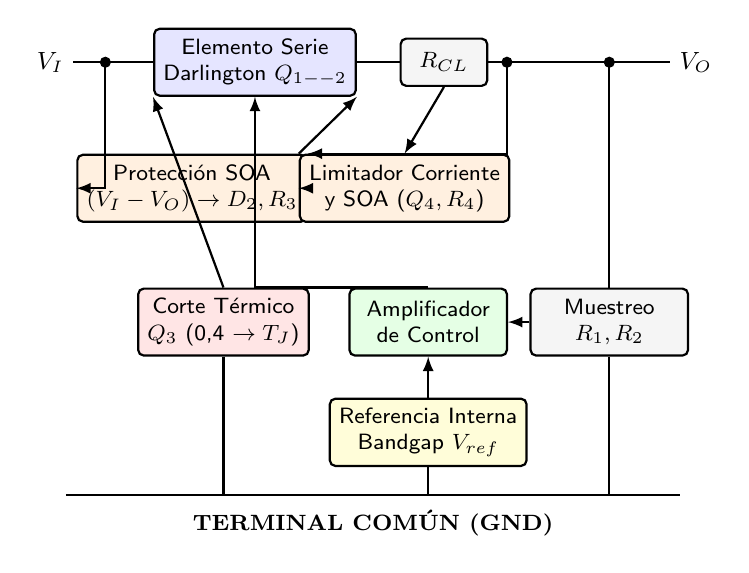
\begin{tikzpicture}[
    block/.style={draw, thick, rectangle, rounded corners=2pt, minimum height=0.85cm, minimum width=2.0cm, align=center, font=\footnotesize\sffamily, fill=gray!8},
    sum/.style={draw, thick, circle, inner sep=1.5pt, font=\footnotesize},
    line/.style={thick, -latex}
]
    % Nodos de entrada y salida
    \node (vin) at (0, 2.5) [font=\small\bfseries] {$V_I$};
    \node (vout) at (8.2, 2.5) [font=\small\bfseries] {$V_O$};

    % Elemento serie y Rsc
    \node[block, fill=blue!10] (pass) at (2.6, 2.5) {Elemento Serie\\Darlington $Q_{1\text{--}2}$};
    \node[block, minimum width=1.1cm, minimum height=0.6cm] (rsc) at (5.0, 2.5) {$R_{CL}$};

    % Protecciones superiores
    \node[block, fill=orange!12] (soa) at (1.8, 0.9) {Protección SOA\\$(V_I - V_O) \to D_2, R_3$};
    \node[block, fill=orange!12] (ilim) at (4.5, 0.9) {Limitador Corriente\\y SOA ($Q_4, R_4$)};

    % Control, referencia, muestreo y térmica
    \node[block, fill=red!10] (therm) at (2.2, -0.8) {Corte Térmico\\$Q_3$ (\SI{0,4}{\volt} $\to T_J$)};
    \node[block, fill=green!10] (ctrl) at (4.8, -0.8) {Amplificador\\de Control};
    \node[block, fill=yellow!15] (vref) at (4.8, -2.2) {Referencia Interna\\Bandgap $V_{\text{ref}}$};
    \node[block] (samp) at (7.1, -0.8) {Muestreo\\$R_1, R_2$};

    % Conexiones principales
    \draw[thick] (vin) -- (pass.west);
    \draw[thick] (pass.east) -- (rsc.west);
    \draw[thick] (rsc.east) -- (vout);
    \draw[thick] (7.1, 2.5) -- (samp.north);
    \filldraw (7.1, 2.5) circle (1.8pt);
    \filldraw (0.7, 2.5) circle (1.8pt);

    % Conexiones de control y protecciones
    \draw[line] (0.7, 2.5) |- (soa.west);
    \draw[line] (5.8, 2.5) |- (soa.north east);
    \filldraw (5.8, 2.5) circle (1.8pt);
    \draw[line] (soa.east) -- (ilim.west);
    \draw[line] (rsc.south) -- (ilim.north);
    \draw[line] (ilim.north west) -- (pass.south east);

    \draw[line] (samp.west) -- (ctrl.east);
    \draw[line] (vref.north) -- (ctrl.south);
    \draw[line] (ctrl.north) -| (pass.south);
    \draw[line] (therm.north) -- (pass.south west);

    % Línea de masa común (GND)
    \draw[thick] (0.2, -3.0) -- (8.0, -3.0);
    \draw[thick] (therm.south) -- (2.2, -3.0);
    \draw[thick] (vref.south) -- (4.8, -3.0);
    \draw[thick] (samp.south) -- (7.1, -3.0);
    \node at (4.1, -3.35) [font=\footnotesize\bfseries] {TERMINAL COMÚN (GND)};
\end{tikzpicture}%
}
\caption{Diagrama funcional en bloques del regulador monolítico \texttt{LM7805C}, destacando el lazo de regulación y las protecciones de corriente, SOA y temperatura (adaptado de Figs. 6-55 y 6-57 \cite{gonzalez_p3}).}
\label{fig:bloques_7805}
\end{figure}

\subsection{Análisis de la Hoja de Datos y Fundamentación del Rango $V_{in(\text{reg})} = \SI{8}{\volt}\text{--}\SI{12}{\volt}$}
En la Tabla~\ref{tab:datasheet_7805} se sintetizan los parámetros eléctricos y térmicos relevantes del regulador $\mu\text{A7805C}$ / \texttt{LM7805C} en encapsulado TO-220, extraídos de la Figura 6-59 del material teórico \cite{gonzalez_p3, ti_7805}. Dichos parámetros se especifican en la condición nominal de ensayo $V_I = \SI{10}{\volt}$, $I_O = \SI{500}{\milli\ampere}$ y $T_J = \SI{25}{\celsius}$.

\begin{table}[htbp]
\centering
\caption{Características eléctricas y térmicas del regulador \texttt{LM7805C} ($\mu\text{A7805C}$, encapsulado TO-220) \cite{gonzalez_p3}.}
\label{tab:datasheet_7805}
\resizebox{\columnwidth}{!}{%
\begin{tabular}{llccc}
\toprule
\textbf{Parámetro} & \textbf{Condiciones de ensayo} & \textbf{Mín.} & \textbf{Típ.} & \textbf{Máx.} \\
\midrule
Tensión de salida ($V_O$) & $I_O = \SI{5}{\milli\ampere}\text{ a }\SI{1}{\ampere}, T_J = \SI{25}{\celsius}$ & \SI{4,8}{\volt} & \SI{5,0}{\volt} & \SI{5,2}{\volt} \\
Tensión de entrada ($V_I$) & Rango operativo recomendado & \SI{7,0}{\volt} & \SI{10,0}{\volt} & \SI{25,0}{\volt} \\
\textbf{Regulación de línea} & $V_I = \SI{7}{\volt}\text{ a }\SI{25}{\volt}, T_J = \SI{25}{\celsius}$ & --- & \textbf{\SI{3}{\milli\volt}} & \textbf{\SI{100}{\milli\volt}} \\
\textbf{Regulación de línea} & $\mathbf{V_I = \SI{8}{\volt}\text{ \textbf{a} }\SI{12}{\volt}}, T_J = \SI{25}{\celsius}$ & --- & \textbf{\SI{1}{\milli\volt}} & \textbf{\SI{50}{\milli\volt}} \\
Rechazo de ripple ($RR$) & $V_I = \SI{8}{\volt}\text{ a }\SI{18}{\volt}, f = \SI{120}{\hertz}$ & \SI{62}{\deci\bel} & \SI{78}{\deci\bel} & --- \\
Regulación de carga & $I_O = \SI{5}{\milli\ampere}\text{ a }\SI{1,5}{\ampere}, T_J = \SI{25}{\celsius}$ & --- & \SI{15}{\milli\volt} & \SI{100}{\milli\volt} \\
Regulación de carga & $I_O = \SI{250}{\milli\ampere}\text{ a }\SI{750}{\milli\ampere}$ & --- & \SI{5}{\milli\volt} & \SI{50}{\milli\volt} \\
Resistencia de salida ($r_o$) & $f = \SI{1}{\kilo\hertz}, T_J = \SI{0}{\celsius}\text{ a }\SI{125}{\celsius}$ & --- & \SI{0,017}{\ohm} & --- \\
Coeficiente térmico ($\Delta V_O/\Delta T$) & $I_O = \SI{5}{\milli\ampere}, T_J = \SI{0}{\celsius}\text{ a }\SI{125}{\celsius}$ & --- & \SI{-1,1}{\milli\volt\per\celsius} & --- \\
Tensión de \emph{dropout} ($V_{DO}$) & $I_O = \SI{1,0}{\ampere}, T_J = \SI{25}{\celsius}$ & --- & \SI{2,0}{\volt} & --- \\
Corriente de reposo ($I_d$) & $T_J = \SI{25}{\celsius}$ & --- & \SI{4,2}{\milli\ampere} & \SI{8,0}{\milli\ampere} \\
Variación de $I_d$ ($\Delta I_d$) & $V_I = \SI{7}{\volt}\text{ a }\SI{25}{\volt}$ / $I_O = \SI{5}{\milli\ampere}\text{ a }\SI{1}{\ampere}$ & --- & --- & \SI{1,3}{\milli\ampere} / \SI{0,5}{\milli\ampere} \\
Corriente de cortocircuito ($I_{SC}$) & $T_J = \SI{25}{\celsius}$ & --- & \SI{750}{\milli\ampere} & --- \\
Temperatura de juntura ($T_J$) & Rango operativo / Máx. absoluta & \SI{0}{\celsius} & --- & \SI{125}{\celsius} / \SI{150}{\celsius} \\
Resistencia térmica ($\theta_{JC} / \theta_{JA}$) & Encapsulado TO-220 (KCS / KC) & --- & \SI{3,0}{\celsius\per\watt} & \SI{19}{\celsius\per\watt}\text{--}\SI{65}{\celsius\per\watt} \\
\bottomrule
\end{tabular}%
}
\end{table}

El análisis detenido de la Tabla~\ref{tab:datasheet_7805} y de la Sección 6-9-3 del apunte de cátedra \cite{gonzalez_p3} justifica técnica y cuantitativamente por qué no resulta conveniente aplicar los \SI{25}{\volt} de la fuente primaria de manera directa al terminal de entrada del \texttt{LM7805C}, sino que debe incorporarse una etapa previa que sitúe su tensión de entrada $V_{i,\text{reg}}$ dentro del intervalo $[\SI{8}{\volt}, \SI{12}{\volt}]$:
\begin{itemize}
    \item \textbf{Optimización de la regulación de línea estática y dinámica:} Cuando el integrado opera dentro de la ventana central $\SI{8}{\volt} \le V_{i,\text{reg}} \le \SI{12}{\volt}$ (centrada en $V_{i,\text{reg}} \approx \SI{9,5}{\volt}\text{--}\SI{10,0}{\volt}$), la variación de tensión de salida se reduce de \SI{3}{\milli\volt} a \textbf{\SI{1}{\milli\volt} típico} (y el máximo garantizado se reduce a la mitad, de \SI{100}{\milli\volt} a \SI{50}{\milli\volt}). Más aún, dado que la etapa prereguladora estabiliza $V_{i,\text{reg}}$ mediante una referencia Zener, una variación severa en la línea primaria (por ejemplo de \SI{25}{\volt} a \SI{10}{\volt}, $\Delta V_{in} = \SI{15}{\volt}$, o fluctuaciones del $\pm \SI{10}{\percent}$ en torno a \SI{25}{\volt}) se traduce en una variación mínima sobre el nodo $V_{i,\text{reg}}$, logrando un doble efecto regulador en cascada.
    \item \textbf{Margen seguro sobre la tensión de \emph{dropout}:} El límite inferior de \SI{8,0}{\volt} asegura una caída diferencial entrada-salida en el regulador integrado de $V_{i,\text{reg}} - V_O = \SI{8,0}{\volt} - \SI{5,0}{\volt} = \SI{3,0}{\volt} > V_{DO} = \SI{2,0}{\volt}$, impidiendo que el transistor Darlington interno salga de su zona activa incluso ante valles de rizado.
    \item \textbf{Desacoplo térmico y preservación del SOA interno del CI:} Operando directamente a $V_{in} = \SI{25}{\volt}$, el diferencial sobre el \texttt{LM7805C} es $V_{in} - V_O = \SI{20}{\volt}$ (situado exactamente en el límite máximo de condiciones recomendadas de la Tabla~\ref{tab:datasheet_7805}). A una corriente nominal de $I_L = \SI{500}{\milli\ampere}$, el integrado debería disipar $P_{D(\text{7805})} = \SI{20}{\volt} \times \SI{0,5}{\ampere} = \SI{10,0}{\watt}$ (y \SI{20,0}{\watt} para $I_L = \SI{1,0}{\ampere}$), lo cual activa la limitación SOA interna ($D_2$) degradando la capacidad de corriente, además de inducir un fuerte corrimiento térmico de la tensión de salida ($\Delta V_O = \SI{-1,1}{\milli\volt\per\celsius} \cdot \Delta T_J$). Al reducir $V_{i,\text{reg}}$ a $\approx \SI{9,5}{\volt}$, la disipación en el \texttt{LM7805C} cae en más de un \SI{77}{\percent} (a sólo \SI{2,27}{\watt} para \SI{500}{\milli\ampere}), transfiriendo el esfuerzo térmico hacia un transistor discreto externo de potencia fácil de refrigerar.
\end{itemize}
